\documentclass[11pt]{article}
\usepackage[english]{babel}
\usepackage{acl2014}
\usepackage{times}
\usepackage{url}
\usepackage{latexsym}
\usepackage{amsmath}
\usepackage{amssymb}
\usepackage{pgfplots}

\begin{document}
\title{Linear Text Regression on Movie Subtitles}
\author{Brian Bechtel, Jonathan Stites\\
       University of Texas at Austin}
\date{}

\maketitle

\begin{abstract}
\noindent
Plot specific features may be useful in predicting box office revenue of films.
Here we present a method for analyzing movie subtitles as a predictive
feature using Linear Text Regression. We find that subtitles have some predictive
power, though not as much as reviews.
We also discuss alternative features that could be used as extensions of this work 
in the future.
\end{abstract}

\section{Introduction}
\subsection{Background and Motivation}
Text regression is a a useful tool to predict real world values from textual inputs.
In 2010, Joshi et al. used text regression on movie reviews to predict box office revenue.
In their paper they analyzed the performance of using reviews as predictor vs using metadata 
alone (such as budget, number of screens, release date, etc.). They found that text
from reviews could both substitute for and improve over a strong metadata based approach.

A limitation in the methodology of Joshi et al. is that they used features that are only
available late into film's production, such as pre-release movie reviews. A pre-release
review requires a cut of the film, which means much, if not all, of the filming has
finished. Thus, the procedure described by Joshi et al. is limited in that a prediction
can only be made late into the production cycle of a film. At such a late point,
significant investments have already been made in the film and thus a prediction of
revenue is of less use for financial planning.

\subsection{Main Goal}
The main goal of this paper was to try and identify prediction features that occur much
earlier in the film making process. We hypothesized that features that captured a film's
plot directly might be useful for predicting revenue. If such features prove useful as
predictors of revenue, then as a consequence prediction can be done much earlier in the
film making process, greatly improving the utility of the model.

We initially wanted to use the film's script as such a feature, but found 
there were no large sources of movie scripts.
From the sources we were able to identify we were only able to
obtain about $140$ usable movie scripts that overlapped with the Joshi et al. data. 
In retrospect, this makes sense as film scripts are considered
intellectual property, and thus the scripts are not widely available to the public.
This legally murky status, in addition to the small amount of data, led to us not
attempting text regression on movie scripts.

As an alternative to scripts, we decided to use the subtitles for the films instead. The
majority of text in a script is the characters' dialogue, and thus since subtitles contain
all the dialogue of the film, we felt that they were a reasonable proxy for scripts.
Scripts do contain other textual information not in subtitles, such as describing a scene,
which makes subtitles not a perfect substitute for scripts.

\subsection{Summary of Results}
In the following sections we describe our methodology for analyzing the subtitle text
and making predictions of box office revenue. Our findings indicate that subtitles do
not perform as well as movie reviews in predicting revenue, though there is some small
predictive value. In general, our attempt to create an effective model that can be used
earlier in the film making process, as compared to those presented in Joshi et al, was 
unsuccessful. However, since we did find that subtitles had some predictive value, it 
is possible that other plot related features of a film may do better. We discuss some of
these alternative plot features in our section on future work.

\section{Problem Definition}
\subsection{Data}
Joshi et al. made their data set accessible to the public. We retrieved there data
and used it as the source the relevant metadata features, review text, and the gross revenue figures for each movie we analyzed in our experiments. The data was stored as
xml which made extracting the features and review text relatively straightforward.

While processing there data, we 
did find that there were some inconsistencies in metadata features such one movie
have its $\mathsf{running\_time}$ feature listed as "Spanish". These erroneous entries
were not too prevalent however, and when encountered we simply replaced them with
sensible defaults. Our process for deciding the defaults is elaborated on more in the
next section.

As mentioned in the introduction, we initally tried to collect script data. We tried
gathering scripts from IMSDb.com, as well as a few other sources, but were only able
to obtain 139 scripts that belonged to the movies in the Josh et al. data set. We then
decided to fall back on using subtitles as the main plot describing feature instead.

We used $\mathsf{subliminal}$, a python CLI program, to download the appropriate
subtitles. $\mathsf{subliminal}$ uses OpenSubtitles.org as the main source of subtitle
data. Once we obtained the subtitles we cleaned them of irrelevant text, such as time
stamps, until only the dialogue text was left. We also sample $5$\% of the subtitles to
verify that they indeed belonged to the correct movie. All subtitles that were manually
checked were correct, which gave us confidence that the $\mathsf{subliminal}$ program
had correctly retrieved the subtitles. Out of the $1718$ movies in the Joshi
et al. data set, we were able to obtain subtitles for $1345$ (placeholder) of them.
While we would have preferred to get subtitles for every movie, we felt that this was
enough to move forward with our regression experiments. The cleaned subtitles are
publicly available from our code repository.

\subsection{Task Definition}
The task at hand was to evaluate how well plot related features, in our case subtitles,
performed in predicting opening weekend revenue in U.S. dollars. Specifically, given
a film's subtitles (and possibly metadata features) in text form, how well can we
predict the film's opening weekend box office revenue.

We use Linear Text Regression to perform this task, where the response variable $y$ is
the film's oppening weekend revenue, and the subtitles and metadata features are
converted into a feature matrix $X$.

\subsection{Algorithm Definition}
We use the Guassian family of linear models as the basis for our prediction method.
Given a response variable $y$, and a feature vector $\vec{x} \in \mathbb{R}^p$, we
predict a value $\hat{y} = \beta_0 + \vec{x}^T \beta$. The parameter $\beta$ and $\beta$
is learned by minimizing the sum of squares errors of the training set.

More specifically we use the Elastic Net model which is a regularized regression method
that linearly combines the penalties from the Lasso and Ridge methods. Let the training
set contain $N$ pairs $x_i,y_i$, where $x_i \in \mathbb{R}^p$ and $y_i \in \mathbb{R}$,
then the Elastic Net equation is as follows:

$$ \min_{(\beta_0, \beta) \in \mathbb{R}^{p+1}} \frac{1}{2N} \sum_{i=1}^N \left(
(y_i - \beta_0 - \vec{x}_i^T\beta)^2 + \lambda P(\beta)\right)$$

\noindent where $\lambda \geq 0$ is a complexity parameter. The penalty term $P(\beta)$
is defined as follows:
$$P(\beta) = \frac{1}{2}(1 - \alpha) \| \beta \|_2^2 + \alpha \|\beta\|_1$$

\noindent where $0 \leq \alpha \leq 1$ is compromise between Ridge ($\alpha = 0$) and
Lasso ($\alpha = 1$) regularization.

Coordinate descent is applied to solve the problem of picking the minimum $\beta_0$ and
$\beta$. Our implementation uses the python package $\mathsf{sklearn}$ which which
contains efficient libraries for training an Elastic Net model using coordinate descent
with cross validation. The hyper parameters $\alpha$ and $\lambda$ are tuned on the dev
data set.

\section{Experimental Evaluation}
\subsection{Methodology}
Our goal was test the effectiveness of subtitles in predicting box office revenue.
To that end, we replicated a portion of the experiments done by Joshi et al. using
movie reviews to use as a baseline for our comparison. We then ran the same set of
experiments substituting subtitles for the movie reviews. This way we could directly
compare the relative performance of subtitles over movie reviews.

Our allocation of training, dev, and test sets differed from Joshi et al.'s in a few
respects. Rather than breaking up the training data into training and dev by year
(2005-2007, 2008, respectively), we simply used 3-fold cross-validation on a training
set (2005-2008). We agreed that it made sense to test the model against movies that were
set in the future from the training data. After all, this model is intended to predict
the opening revenue of future movies. However, we were skeptical that this was necessary
for good cross-validation.

In the experiments we used both text features and metadata features. The metadata features
we selected were the release date, whether the movie was domestic or foreign, the production
budget, the number of screens, the film's rating, the genre of the film, and its running
time. This is a strict subset of the metadata used by Joshi et al. We left out some of the
metadata features they used such as 'number of oscar winning actors' as the data set they
provided was inconsistent in recording such features. We felt the meta data features they
we did use was a good sampling of the most predictive features available.

We used $n$-grams as the basis for extracting text features. This corresponds to type
$I$ text features extracted by Joshi et al. In the case of reviews, we combined
each review for a movie into one large document when extracting text features. In the
case of subtitles there was only one document per film. Before extracting $n$-grams we
preprocessed the documents using common NLP techniques. This consisted of converting
the text to lower case, removing punctuation, and removing $n$-grams that occured in all documents. 
Once the documents
had been preprocessed we extracted various types of $n$-grams depending upon the
experiment type. We considered using unigrams alone, unigrams + bigrams, unigrams +
bigrams + trigrams, bigrams + trigrams, and trigrams alone. Additionally, we used at most
the top 10,000 entries per $n$-gram type. This adds to at most 30,000 features in when using
unigrams, bigrams, and trigrams. Joshi et al. did no filtering on by ngram frequency.

We evaluated our models using mean absolute error (MAE) and $r^2$ of weekend gross revenue
and of United States gross revenue. 

\begin{table*}[t]
\caption{Experiment Results for Unigrams + Bigrams with a Max Feature Size of 10,000}
\centering
\begin{tabular}{|l c c c c|}
  \hline
  \textbf{Experiment} & \textbf{MAE WG (\$M)} & \textbf{$r^2$ WG} & \textbf{MAE USG (\$M)}
  & \textbf{$r^2$ USG}\\
  \hline
  metadata                    &  7.061 &  0.471  & 22.010  & 0.497\\
  reviews                     &  8.444 &  0.518  & 27.290  & 0.353\\
  subtitles                   & 10.345 &  0.085  & 32.554  & 0.095\\
  reviews+subtitles           &  8.310 &  0.526  & 27.179  & 0.394\\
  metadata+reviews            &  6.969 &  0.450  & 21.583  & 0.486\\
  metadata+subtitles          &  7.062 &  0.468  & 22.000  & 0.496\\
  metadata+reviews+subtitles  &  6.972 &  0.464  & 22.093  & 0.496\\
  \hline
  \multicolumn{5}{l}{\textsuperscript{*}\footnotesize{WG: weekend gross revenue. USG:
  United States Gross Revenue}}
\end{tabular}
\end{table*}

\subsection{Results}
Present the quantitative results of your experiments. Graphical data presentation such as
graphs and histograms are frequently better than tables. What are the basic differences
revealed in the data. Are they statistically significant?

\begin{figure}[h]
\resizebox {\columnwidth} {!} {
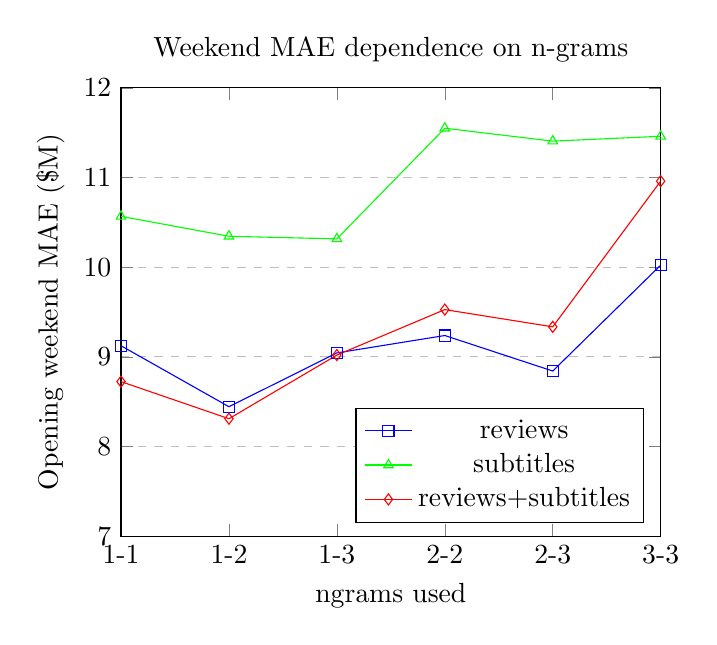
\begin{tikzpicture}
\begin{axis}[
    title={Weekend MAE dependence on n-grams},
    xlabel={ngrams used},
    ylabel={Opening weekend MAE (\$M)},
    xmin=1, xmax=6,
    ymin=7, ymax=12,
    xtick={1,2,3,4,5,6},
    xticklabels={1-1,1-2,1-3,2-2,2-3,3-3},
    ytick={7,8,9,10,11,12},
    legend pos=south east,
    ymajorgrids=true,
    grid style=dashed,
]
 
\addplot[
    color=blue,
    mark=square,
    ]
    coordinates {
    (1,9.124)(2,8.444)(3,9.044)(4,9.238)(5,8.842)(6,10.023)
    };
    \legend{reviews}

\addplot[
    color=green,
    mark=triangle,
    ]
    coordinates {
    (1,10.567)(2,10.345)(3,10.316)(4,11.550)(5,11.406)(6,11.460)
    };
    \addlegendentry{subtitles}
    
\addplot[
    color=red,
    mark=diamond,
    ]
    coordinates {
    (1,8.724)(2,8.310)(3,9.020)(4,9.527)(5,9.335)(6,10.960)
    };
    \addlegendentry{reviews+subtitles}
 
\end{axis}
\end{tikzpicture}
}
\end{figure}

\begin{figure}[h]
\resizebox {\columnwidth} {!} {
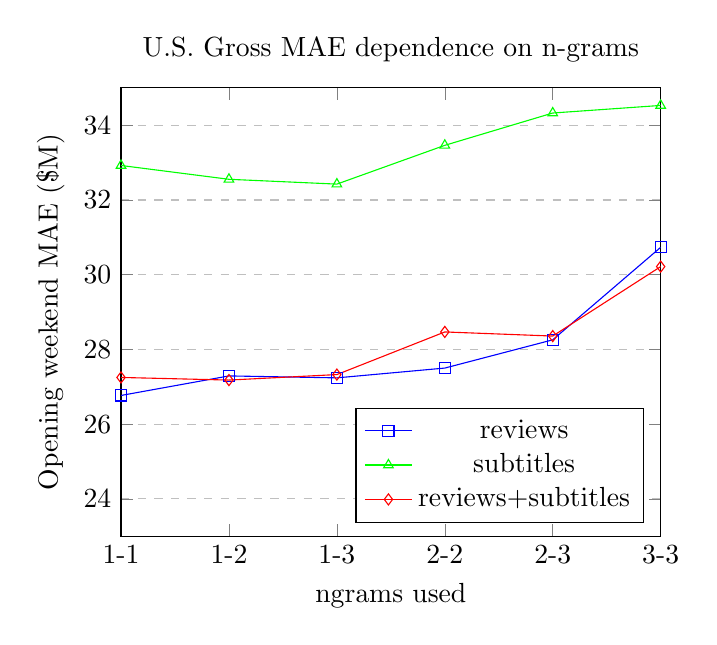
\begin{tikzpicture}
\begin{axis}[
    title={U.S. Gross MAE dependence on n-grams},
    xlabel={ngrams used},
    ylabel={Opening weekend MAE (\$M)},
    xmin=1, xmax=6,
    ymin=23, ymax=35,
    xtick={1,2,3,4,5,6},
    xticklabels={1-1,1-2,1-3,2-2,2-3,3-3},
    ytick={24,26,28,30,32,34},
    legend pos=south east,
    ymajorgrids=true,
    grid style=dashed,
]
 
\addplot[
    color=blue,
    mark=square,
    ]
    coordinates {
    (1,26.767)(2,27.290)(3,27.238)(4,27.500)(5,28.256)(6,30.732)
    };
    \legend{reviews}

\addplot[
    color=green,
    mark=triangle,
    ]
    coordinates {
    (1,32.923)(2,32.553)(3,32.424)(4,33.462)(5,34.327)(6,34.530)
    };
    \addlegendentry{subtitles}
    
\addplot[
    color=red,
    mark=diamond,
    ]
    coordinates {
    (1,27.249)(2,27.179)(3,27.326)(4,28.467)(5,28.357)(6,30.216)
    };
    \addlegendentry{reviews+subtitles}
 
\end{axis}
\end{tikzpicture}
}
\end{figure}

\subsection{Discussion}
Our hypothesis that movie subtitles could be used to predict the weekend gross revenue
was confirmed. However, the predictive power is weak and unlikely
to be useful in practice. 

Our original hypothesis, that scripts would have predictive power, is based on
the idea that plot matters. However, subtitles are very imperfect proxies for plot. 
Therefore, we think that there is simply not very much information to be gained from
scripts. 

If a movie studio could be convinced to release a bulk collection of movie scripts,
then perhaps a model could be trained on scripts and be useful practice.

Additionally, linear text regression treats the documents as a bag of words. While
this can be useful, as in the case of reviews, it does preclude the ability of the
model to "learn" about a movie's plot. 


\section{Related Work}
Joshi et al. (2010) is the main basis for our paper. In their paper they describe their
technique to use Linear Text Regression on movie reviews to predict box office revenue.
Their work is based on sentiment analysis of Pang et al. (2002) and the uses of critic
reviews of Terry et al. (2005). The main difference in the work of Joshi et al. is that
they considered the review text directly rather than sentiment, number of start, etc. as
well as using the analysis to predict future real valued quantities. Prior work had
used all data including those past the release of the movie to predict revenue. Joshi
et al. limited themselves to data that was available only prior to the films's release.
Our work is an extension of Joshi et al. in that we are using text features, i.e.
subtitles, that are available much earlier in the film making process. Given the results
of our experiments it is hard to say if our method is strictly better than that proposed
by Joshi et al. However, since we did find some predictive value in using the text of
subtitles, our method may have marginal utility over that of Joshi et al. in that our
method allows a prediction much sooner than their method.

Bitvai et al. (2015) extended the work of Joshi et al. They used the data set and
features described by Joshi et al, but instead of using a linear model they apply
a non-linear method based on a deep convolutional neural network. They reported a 40\%
relative improvement over sparse linear models. The work of Bitvai et al. is parallel to
ours in that both our work and that of Bitvai et al are extension of the method described
by Joshi et al. The key difference is that they enhanced the underlying model of Joshi
et al. while our enhancement centered around using text features available earlier
in the film making process. The strength of the improvement reported by Bitvai et al. 
indicates that their enhancement is likely better than ours, however their enhancement is
in an orthogonal direction to direction making it unclear how to do a direct comparison.
It would be interesting to combine the work of Bitvai et al. with ours to see if a
convolutional neural network can use subtitles more effectively than a linear model.

\section{Future Work}
The first major weakness of our work is that we had to rely on using subtitles as the
major plot related textual feature. As previously mentioned, our initial desire was to
use the film's scripts but we had to abandon that approach as there was not enough
movie script data to use. If sufficient script data could be obtained a potential
enhancement would be to substitute script data for the subtitle data we used.

A second potential enhancement, related to the first, is to experiment with other
plot related text features. For example plot summaries could be used instead of subtitles.
The relatively weak performance of subtitles could be from a low signal to noise ratio
where much of the predictive information is lost to irrelevant data. A more concise
description of the plot, such as a plot summary, may have a higher signal to noise ratio.
A good extension of our work would be to test if such concise plot features have higher
predictive power.

Another weakness is that we did not change the underlying predictive model. We still
used linear regression even though better text regression models have been developed in
recent years. We felt that using a linear model was fine because our main goal was to
test the predictive power of plot related features. Since our results did indicate small
predictive element an nice improvement over our work would be to improve the underlying
predictive model to test if more relevant information can be extracted from subtitles.
The work done by Bitvai et al using convolutional neural networks would be a natural place
to start with this type of enhancement. 

\section{Conclusion}
For the task of predicting box office revenue through text regression, subtitles
substantially under perform other text features such as movie reviews. However,
subtitles do have some predictive power, indicating the features related to a film's plot
do have an impact on revenue generated. It seems worth while to investigate other
features related to plot, such as plot summaries, in future work to evaluate how well
plot features perform in general.

\begin{thebibliography}{9}

\bibitem{Bitvai2015}
  Zsolt Bitvai, Trevor Cohn,
  Non-Linear Text Regression with a Deep Convolutional Neural Network,
  Proceedings of the 53rd Annual Meeting of the Association for Computational
  Linguistics and the 7th International Joint Conference on Natural Language Processing,
  2015.
    
\bibitem{Joshi2010}
  Mahesh Joshi, Dipanjan Das, Kevin Gimpel, Noah A. Smith,
  Movie Reviews and Revenues: An Experiment in Text Regression,
  Proceedings of NAACL-HLT,
  2010.
  
\bibitem{Pang2002}
  Bo Pang, Lillian Lee, Shivakumar Vaithyanathan,
  Thumbs up? Sentiment Classification using Machine Learning Techniques,
  Proceedings of EMNLP,
  2002.
  
\bibitem{Terry2002}
  Neil Terry, Michael Butler, De'Arno De'Armond,
  The Determinants of Domestic Box Office Performance In the Motion Picture Industry,
  Southwestern Economic Review,
  2005.
    
\bibitem{JoshiData}
  Mahesh Joshi, Dipanjan Das, Kevin Gimpel, Noah A. Smith,
  "Movie Data",
  Web,
  Accessed 04 May 2017,
  https://www.cs.cmu.edu/~ark/movie\$-data/

\bibitem{IMSDb}
    "The Internet Movie Script Database",
    Web,
    Accessed 14 April 2017,
    http://www.imsdb.com/disclaimer/
    
\bibitem{Subliminal}
    "Subliminal: python library to search and download subtitles",
    Web,
    Accessed 04 May 2017,
    https://subliminal.readthedocs.io/en/latest/r/
  
\end{thebibliography}
\end{document}
%%% Local Variables: 
%%% mode: latex
%%% TeX-master: t
%%% End: 

